\documentclass{article}

\usepackage{graphicx}
\usepackage{rotating}
\usepackage{amsmath}
\usepackage{fancyhdr}
\usepackage{listings}
\usepackage{xcolor}
\usepackage{color}
\usepackage{textcomp}
\usepackage{float}
\usepackage{multirow}
\usepackage[sorting=none]{biblatex}
\usepackage[margin=1in]{geometry}
\usepackage[font={small,it}]{caption}
\usepackage{placeins}
\usepackage{xepersian}

%\DeclareMathOperator*{\btie}{\bowtie}
\addbibresource{bibliography.bib}
\settextfont[Scale=1.2]{B-NAZANIN.TTF}
\setlatintextfont[Scale=1]{Times New Roman}
\renewcommand{\baselinestretch}{1.5}
\pagestyle{fancy}
\fancyhf{}
\rhead{تکلیف پنجم درس مبانی بینایی کامپیوتر}
\lhead{\thepage}
\rfoot{علیرضا ابره فروش}
\lfoot{9816603}
\renewcommand{\headrulewidth}{1pt}
\renewcommand{\footrulewidth}{1pt}
%%%%%%%%%%
\lstset
{
    language=[latex]tex,
    basicstyle=\ttfamily,
    commentstyle=\color{black},
    columns=fullflexible,
    keepspaces=true,
    upquote=true,
    showstringspaces=false,
    morestring=[s]\\\%,
    stringstyle=\color{black},
}
%%%%%%%%%%
%beginMatlab
\definecolor{mygreen}{RGB}{28,172,0} % color values Red, Green, Blue
\definecolor{mylilas}{RGB}{170,55,241}
%endMatlab
\begin{document}
%beginMatlab
\lstset{language=Matlab,%
    %basicstyle=\color{red},
    breaklines=true,%
    morekeywords={matlab2tikz},
    keywordstyle=\color{blue},%
    morekeywords=[2]{1}, keywordstyle=[2]{\color{black}},
    identifierstyle=\color{black},%
    stringstyle=\color{mylilas},
    commentstyle=\color{mygreen},%
    showstringspaces=false,%without this there will be a symbol in the places where there is a space
    numbers=left,%
    numberstyle={\tiny \color{black}},% size of the numbers
    numbersep=9pt, % this defines how far the numbers are from the text
    emph=[1]{for,end,break},emphstyle=[1]\color{red}, %some words to emphasise
    %emph=[2]{word1,word2}, emphstyle=[2]{style},    
}
%endMatlab
\begin{titlepage}
\begin{center}

\includegraphics[width=0.4\textwidth]{figures/IUT Logo.png}\\
        
\LARGE
\textbf{دانشگاه صنعتی اصفهان}\\
\textbf{دانشکده مهندسی برق و کامپیوتر}\\
        
\vfill
        
\huge
\textbf{عنوان: تکلیف چهارم درس ریزپردازنده}\\
        
\vfill
        
\LARGE
\textbf{نام و نام خانوادگی: علیرضا ابره فروش}\\
\textbf{شماره دانشجویی: 9816603}\\
\textbf{نیم\,سال تحصیلی: پاییز 1400}\\
\textbf{مدرّس: دکتر عارف کریمی افشار}\\
\end{center}
\end{titlepage}


%\tableofcontents
\newpage


\section{}%1
از آنجایی که این نسخه از $LBP$ یکنواخت است تعداد \lr{transition}ها در الگوی باینری به دست آمده حداکثر 2 است. همچنین ناوردا بودن آن نسبت به چرخش باعث می‌شود که این حالت‌ها صرفا در تعداد صفر (یا یک) با یکدیگر تفاوت داشته باشند. به مثال زیر برای $LBP_{8,1}^{riu2}$ توجه کنید.
\begin{figure}[H]
    \centering
    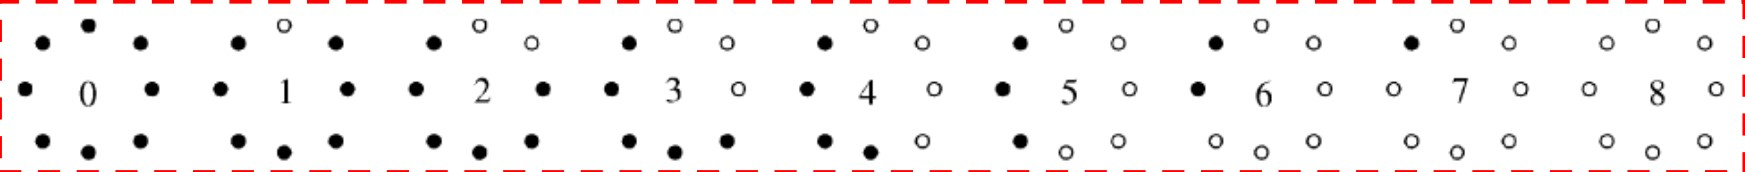
\includegraphics[width=1.0\textwidth]{figures/1.jpg}
    \caption
	{
الگوهای مختلف در $LBP_{P,R}^{riu2}$
	}
    \label{fig:fig1}
\end{figure}
همانطور که می‌بینیم تعداد بین‌ها در $LBP_{8,1}^{riu2}$ برابر با 10 خواهد بود. پس به ازای $LBP_{P,R}^{riu2}$ تعداد صفرها از $0$ تا $P$ می‌تواند متغیر باشد. تعداد بین‌های هیستوگرام برابر با تعداد حالات مختلف این الگوها به علاوه‌ی یک (برای همه‎ی الگوهای غیریکنواخت یک بین در نظر می‌گیریم) است. پس تعداد بین‌ها در هسیتوگرام نظیر آن برابر
$P+2$
خواهد بود.

\section{}%2
\subsection{الف}
\subsubsection{\lr{Algorithm}}
برای شمارش سلول به صورت بازگشتی عمل می‌کنیم. به ازای هر پیکسل سفید آن را سیاه می‌کنیم و سپس الگوریتم را روی پیکسل‌های سفید در همسایگی 3 در 3 آن اجرا می‌کنیم. اگر همسایه‌ی سفید نداشت یکی به شمارش‌گر سلول‌ها اضافه می‌شود. این کار را تا جایی ادامه می‌دهیم که همه‌ی پیکسل‌ها پیمایش شوند (هیچ پیکسل سفیدی در تصویر باقی نماند). برای رفع مشکل یکی شمرده شدن سلول‌های به هم چسبیده از عملگر \lr{erosion} با المان ساختاری دایره به شعاع 5 استفاده می‌کنیم.

\subsubsection{\lr{Function}}
\begin{latin}
\lstinputlisting{sources/countCells.m}
\end{latin}

\subsubsection{\lr{Driver code}}
\begin{latin}
\lstinputlisting{sources/p2a.m}
\end{latin}


\subsection{ب}

\subsubsection{\lr{Algorithm}}
برای برچسب‌گذاری سلول‌ها و نهایتا محسابه‌ی مساحت و میانگین سطح روشنایی آن‌ها به صورت بازگشتی عمل می‌کنیم. یک \lr{map} (ماتریس هم‌اندازه با تصویر ورودی) نظیر تصویر ورودی که درواقع برچسب هر پیکسل (که در کدام ناحیه قرار دارد) می‌سازیم. به ازای هر پیکسل سفید در \lr{map} پیکسل نظیر آن را برچسب می‌دهیم و آن را سیاه می‌کنیم و سپس الگوریتم را روی پیکسل‌های سفید در همسایگی 3 در 3 آن اجرا می‌کنیم. اگر همسایه‌ی سفید نداشت یکی به شمارش‌گر ناحیه اضافه می‌شود. این کار را تا جایی ادامه می‌دهیم که همه‌ی پیکسل‌ها پیمایش شوند (هیچ پیکسل سفیدی در تصویر باقی نماند).

\subsubsection{\lr{Function}}
\begin{latin}
\lstinputlisting{sources/saveCellsData.m}
\end{latin}

\subsubsection{\lr{Driver code}}
\begin{latin}
\lstinputlisting{sources/p2b.m}
\end{latin}



\section{}%3
\subsection{\lr{Block diagram}}
\begin{figure}[H]
    \centering
    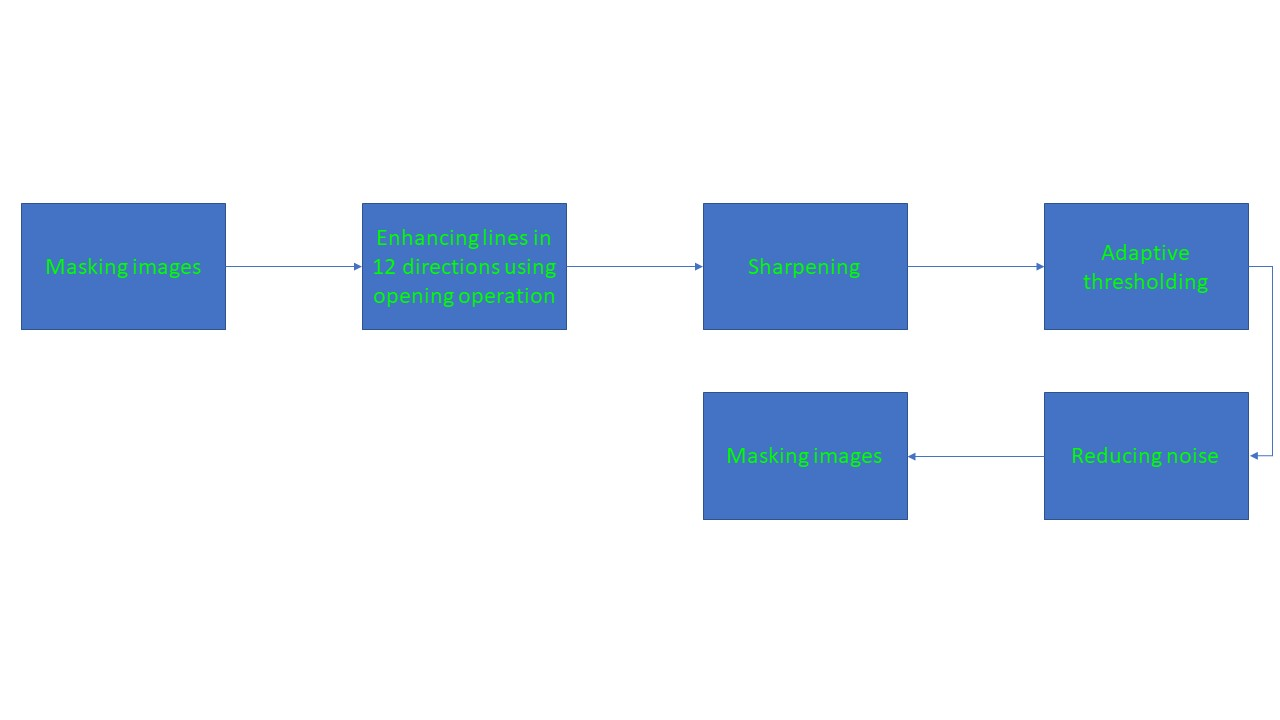
\includegraphics[width=1.0\textwidth]{figures/3.jpg}
    \caption
	{
بلوک‌دیاگرام روش پیاده‌سازی شده
	}
    \label{fig:fig1}
\end{figure}

\subsection{\lr{Algorithm}}
ابتدا ماسک تصاویر را اعمال می‌کنیم تا حاشیه‌ی آن‌ها کاملا سیاه شود. سپس به وسیله‌ی عملگر \lr{opening} و با المان ساختاری خط به طول 7، خطوط را در 12 جهت مختلف تقویت می‌کنیم تا هم رگ‌های ریز نمایان‌تر شوند و هم نویز‌های غیرخطی گرفته شوند. سپس تصویر را به وسیله‌ی \lr{unsharp masking} شارپ می‌کنیم. با استفاده از روش آستانه‌گذاری وفقی تصویر را به تصویر سیاه‌سفید تبدیل می‌کنیم. جهت تقویت رگ‌ها روی تصویر عملگر \lr{dilation} با المان ساختاری خط به طول 6 در راستای افقی اعمال می‌کنیم. در نهایت به وسیله‌ی فیلتر میانه نویز را کاهش می‌دهیم.

\subsection{\lr{Driver code}}
\begin{latin}
\lstinputlisting{sources/p3.m}
\end{latin}

\subsection{\lr{Results}}
\subsubsection{پزشک اول}
%table
\begin{latin}
\begin{table}[H]
\begin{tabular}{|c|c|c|c|}
\hline
\textbf{\lr{Accuracy}} & \textbf{\lr{Specificity}} & \textbf{\lr{Sensitivity}} & \textbf{}             \\ \hline
90.66                  & 91.25                     & 84.63                     & \textbf{1}            \\ \hline
91.25                  & 91.98                     & 84.91                     & \textbf{2}            \\ \hline
88.82                  & 89.56                     & 82.08                     & \textbf{3}            \\ \hline
89.65                  & 90.14                     & 84.80                     & \textbf{4}            \\ \hline
90.12                  & 91.06                     & 81.07                     & \textbf{5}            \\ \hline
90.84                  & 92.45                     & 75.93                     & \textbf{6}            \\ \hline
89.69                  & 90.50                     & 81.64                     & \textbf{7}            \\ \hline
89.99                  & 91.07                     & 78.50                     & \textbf{8}            \\ \hline
92.22                  & 94.13                     & 70.59                     & \textbf{9}            \\ \hline
88.65                  & 89.21                     & 82.50                     & \textbf{10}           \\ \hline
89.73                  & 90.65                     & 80.45                     & \textbf{11}           \\ \hline
90.03                  & 90.84                     & 81.42                     & \textbf{12}           \\ \hline
90.69                  & 92.19                     & 76.80                     & \textbf{13}           \\ \hline
89.47                  & 89.75                     & 86.25                     & \textbf{14}           \\ \hline
80.02                  & 79.03                     & 92.87                     & \textbf{15}           \\ \hline
90.67                  & 0.9191                    & 78.25                     & \textbf{16}           \\ \hline
92.08                  & 93.96                     & 71.68                     & \textbf{17}           \\ \hline
91.30                  & 92.43                     & 78.18                     & \textbf{18}           \\ \hline
87.27                  & 87.09                     & 89.26                     & \textbf{19}           \\ \hline
90.66                  & 91.23                     & 83.40                     & \textbf{20}           \\ \hline
\textbf{89.69}         & \textbf{90.52}            & \textbf{81.26}            & \textbf{\lr{Average}} \\ \hline
\end{tabular}
\end{table}
\end{latin}
%table
\subsubsection{پزشک دوم}
%table
\begin{latin}
\begin{table}[H]
\begin{tabular}{|c|c|c|c|}
\hline
\textbf{\lr{Accuracy}} & \textbf{\lr{Specificity}} & \textbf{\lr{Sensitivity}} & \textbf{}             \\ \hline
90.68                  & 91.18                     & 85.45                     & \textbf{1}            \\ \hline
91.48                  & 92.03                     & 86.62                     & \textbf{2}            \\ \hline
88.93                  & 89.16                     & 86.58                     & \textbf{3}            \\ \hline
89.50                  & 89.86                     & 85.72                     & \textbf{4}            \\ \hline
90.35                  & 90.63                     & 87.24                     & \textbf{5}            \\ \hline
90.54                  & 92.09                     & 75.51                     & \textbf{6}            \\ \hline
89.26                  & 89.41                     & 87.38                     & \textbf{7}            \\ \hline
89.71                  & 90.07                     & 84.71                     & \textbf{8}            \\ \hline
92.02                  & 94.01                     & 69.42                     & \textbf{9}            \\ \hline
88.63                  & 88.75                     & 87.12                     & \textbf{10}           \\ \hline
90.07                  & 90.55                     & 84.81                     & \textbf{11}           \\ \hline
90.04                  & 90.58                     & 83.86                     & \textbf{12}           \\ \hline
90.56                  & 92.28                     & 75.24                     & \textbf{13}           \\ \hline
89.34                  & 89.42                     & 88.36                     & \textbf{14}           \\ \hline
80.20                  & 79.22                     & 92.36                     & \textbf{15}           \\ \hline
91.12                  & 91.91                     & 82.60                     & \textbf{16}           \\ \hline
92.69                  & 93.79                     & 78.84                     & \textbf{17}           \\ \hline
92.10                  & 93.46                     & 78.63                     & \textbf{18}           \\ \hline
87.97                  & 88.15                     & 86.35                     & \textbf{19}           \\ \hline
90.72                  & 92.13                     & 76.85                     & \textbf{20}           \\ \hline
\textbf{89.80}         & \textbf{83.18}            & \textbf{83.18}            & \textbf{\lr{Average}} \\ \hline
\end{tabular}
\end{table}
\end{latin}
%table


%%%%%%%%%%%%%%%%%%%%%%%%%%%%%%%%%%%


%\begin{latin}
%\lstinputlisting{sources/p1.m}
%\end{latin}

%\begin{figure}[H]
%    \centering
%    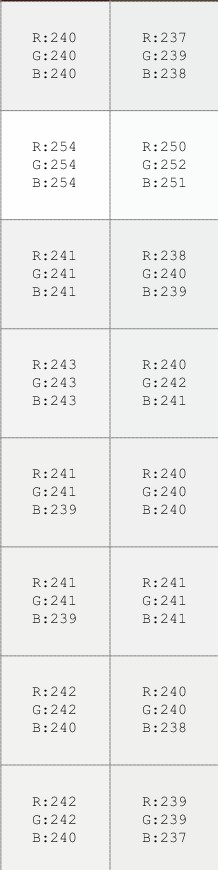
\includegraphics[width=0.25\textwidth]{figures/5p3.jpg}
%    \caption
%	{
%لبه‌ها (نمای نزدیک)
%	}
%    \label{fig:fig1}
%\end{figure}


%%%%%%%%%%%%%%%%%%%%%%%%%%%%%%%%%%%
%%%%%%%%%%%%%%%%%%%%%%%%%%%%%%%%%%%
%%%%%%%%%%%%%%%%%%%%%%%%%%%%%%%%%%%

%------------------------------------------------------------------------------------------


\section*{منابع}
\renewcommand{\section}[2]{}%
\begin{thebibliography}{99} % assumes less than 100 references
%چنانچه مرجع فارسی نیز داشته باشید باید دستور فوق را فعال کنید و مراجع فارسی خود را بعد از این دستور وارد کنید


\begin{LTRitems}

\resetlatinfont

\bibitem{b1}
\end{LTRitems}

\end{thebibliography}


\end{document}
